% Created 2021-03-03 mié 21:21
% Intended LaTeX compiler: pdflatex
\documentclass[presentation,aspectratio=169]{beamer}
\usepackage[utf8]{inputenc}
\usepackage[T1]{fontenc}
\usepackage{graphicx}
\usepackage{grffile}
\usepackage{longtable}
\usepackage{wrapfig}
\usepackage{rotating}
\usepackage[normalem]{ulem}
\usepackage{amsmath}
\usepackage{textcomp}
\usepackage{amssymb}
\usepackage{capt-of}
\usepackage{hyperref}
\usepackage{khpreamble}
\usepackage{amssymb}
\usepgfplotslibrary{groupplots}
\newcommand*{\shift}{\operatorname{q}}
\DeclareMathSymbol{\Omega}{\mathalpha}{letters}{"0A}% italics
\DeclareMathSymbol{\varOmega}{\mathalpha}{operators}{"0A}% upright
\providecommand*{\upOmega}{\varOmega}% for siunitx
\usepackage[binary-units=true]{siunitx}
\usepackage{circuitikz}
\usetheme{default}
\author{Kjartan Halvorsen}
\date{2021-03-01}
\title{Actuadores}
\hypersetup{
 pdfauthor={Kjartan Halvorsen},
 pdftitle={Actuadores},
 pdfkeywords={},
 pdfsubject={},
 pdfcreator={Emacs 26.3 (Org mode 9.4.4)}, 
 pdflang={English}}
\begin{document}

\maketitle

\section{Requerimientos mecanicos}
\label{sec:org464a193}

\begin{frame}[label={sec:org3c3041c}]{Requerimientos mecanicos}
\end{frame}
\begin{frame}[label={sec:org96f87b0}]{Energía mecánica}
From Encyclopaedia Britannica
\begin{quote}
\alert{Energía mecánica} La suma de energía cinética (energía de movimiento) y la energía potencial (energía almacenada en una sistema por la posición de sus partes).
\end{quote}

\[ E_M = \underbrace{K}_{\text{Energía cinética}} + \underbrace{U}_{\text{Energía potencial}}\]

Una masa \(m\) con velocidad \(v\) a una altura \(h\) sobre un nivel de referéncia, tiene la energía mecánica \(E_M = \frac{1}{2}mv^2 + mgh\).

\begin{center}
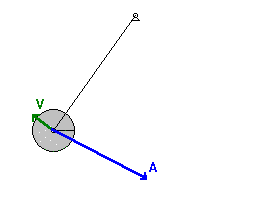
\includegraphics[height=0.3\textheight]{../../figures/pendulum.png}
{\footnotesize Fuente: Hubert Christiaen, wikipedia}
\end{center}


\#+end\textsubscript{center}
\end{frame}
\begin{frame}[label={sec:org55e5e47}]{Trabajo}
From Encyclopaedia Britannica
\begin{quote}
\alert{Trabajo} En la físisca, la medida de \alert{transferencia de energía} que ocurre cuando un objeto está desplazado \alert{una distancia} por una \alert{fuerza externa} cuya tiene un componente en la dirección del desplazamiento.
\end{quote}
\end{frame}

\begin{frame}[label={sec:org6572bb4}]{Trabajo}
\begin{center}
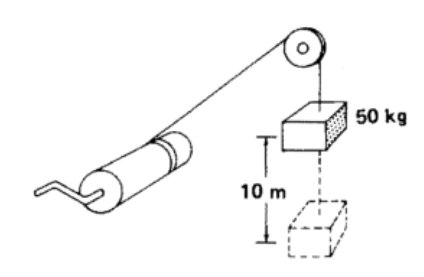
\includegraphics[height=0.6\textheight]{../../figures/pulley-block-50kg.png}
\end{center}

\alert{Actividad individual 1} Se sube un cuerpo de \unit{50}{\kilogram} una distancia de \unit{10}{\meter}. Calcula el trabajo realizado. Manda tu respuesta en el chat.
\end{frame}



\begin{frame}[label={sec:org585b1c9}]{Potencia}
\alert{Definición} La derivada del tiempo del trabajo.
\end{frame}

\begin{frame}[label={sec:org21f0b99}]{Potencia}
\begin{center}
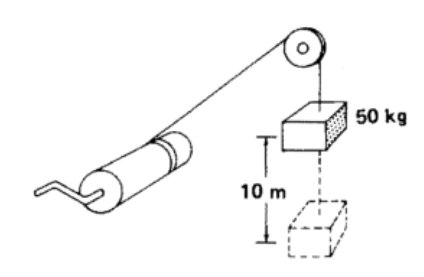
\includegraphics[height=0.6\textheight]{../../figures/pulley-block-50kg.png}
\end{center}

\alert{Actividad individual 2} Se subió un cuerpo de masa \unit{50}{\kilogram}  a una distancia de \unit{10}{\meter} en \unit{5}{\second}. Determine la potencia promedia. Se ignora la fricción.
\end{frame}

\begin{frame}[label={sec:orgd3dc50b}]{Potencia y fuerza para accelerar}
   \begin{center}
\begin{tikzpicture}

  \begin{scope}[scale=0.3, xshift=4cm]
  \node[anchor=south,] {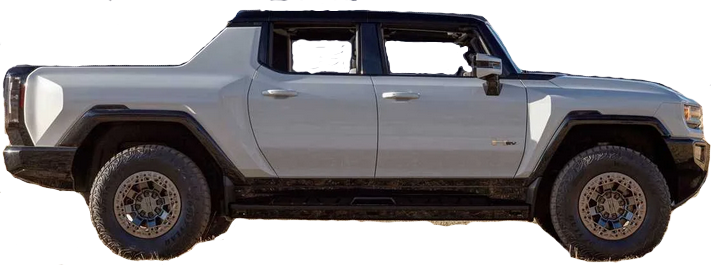
\includegraphics[width=3cm]{../../figures/hummer-ev.png}};
    \draw[thin, ] (-8,2) -- (-6,2);
    \draw[thin, ] (-9,3) -- (-6.5,3);
  \end{scope}

  \draw[->,semithick] (-.5,0.16) -- (8,0.16);
\end{tikzpicture}
\end{center}


\alert{Actividad individual 3} El nuevo Hummer EV tiene una masa de \(m=\unit{5000}{\kilogram}\), y puede accelerarar de \unit{0 - 100}{\kilo\meter\per\hour} en tres segundos. Cual es la potencia promedio necesario para lograr esto (ignorando la resistencia del aire y ra resistencia a la rodura)?
\end{frame}

\begin{frame}[label={sec:orgde875e1}]{Potencia en rotación}
\alert{Torque} por \alert{velocidad angular}

\[ P = T\omega\]
\end{frame}

\begin{frame}[label={sec:org89ac5b6}]{Momento de inercia}
\begin{columns}
\begin{column}{0.38\columnwidth}
\begin{center}
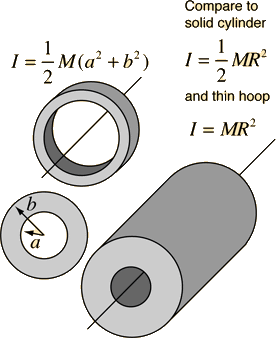
\includegraphics[height=0.6\textheight]{../../figures/moment-of-inertia-cylinder.png}
{\footnotesize Fuente: Georgia State University}
\end{center}
\end{column}

\begin{column}{0.72\columnwidth}
El factor que determine la tendencia de un cuerpo de resistir aceleración angular:
\[ \textcolor{red!80!black}{J} \dot{\omega} = \sum T_i \]
Y la magnitúd de la energía cinética a cierta velocidad angular:
\[ K = \frac{1}{2}\textcolor{red!80!black}{J}\omega^2.\]
\end{column}
\end{columns}
\end{frame}



\begin{frame}[label={sec:org0ac4a5b}]{Requerimientos de potencia y torque para un elevador}
\begin{columns}
\begin{column}{0.38\columnwidth}
\begin{center}
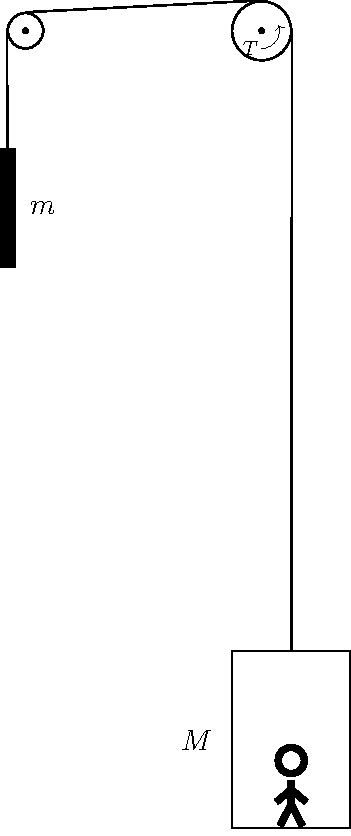
\includegraphics[height=0.8\textheight]{../../figures/mech-elevator}
\end{center}
\end{column}

\begin{column}{0.72\columnwidth}
Dado un elevador de masa \(M=\unit{1000}{\kilogram}\), contrapeso con masa \(m=\unit{800}{\kilogram}\) y poleo con radius of \(r=\unit{0.4}{\meter}\). Un motor eléctrico está conectado al poleo con un reductor de velocidad con relación de transmisión de 12:1 (12 revoluciones del motor para cada revolución del poleo). El rotor tiene un momento de inercia de \(J_m = \unit{0.3}{\kilogram\meter\squared}\). La inercia del poleo se puede ignorar.

 \alert{Actividad en grupo} 
\alert{(a)} ¿A que velocidad angular gira el motor cuando el elevador sube a \unit{4}{\meter\per\second}? \alert{(b)} Determine la potencia y el torque del motor necesario para subir el elevador a \unit{4}{\meter\per\second}. \alert{(c)} El elevador usa dos segundos para llegar a la velocidad \unit{4}{\meter\per\second} desde cero. En este tiempo se ha movido \unit{4}{\meter} hacia arriba. Determine la potencia promedia y el torque promedio durante el arranque.
\end{column}
\end{columns}
\end{frame}

\section{El motor electrico de corriente continua}
\label{sec:orgd8a4f70}
\begin{frame}[label={sec:org0b45881}]{El motor eléctrico de corriente continua}
\begin{center}
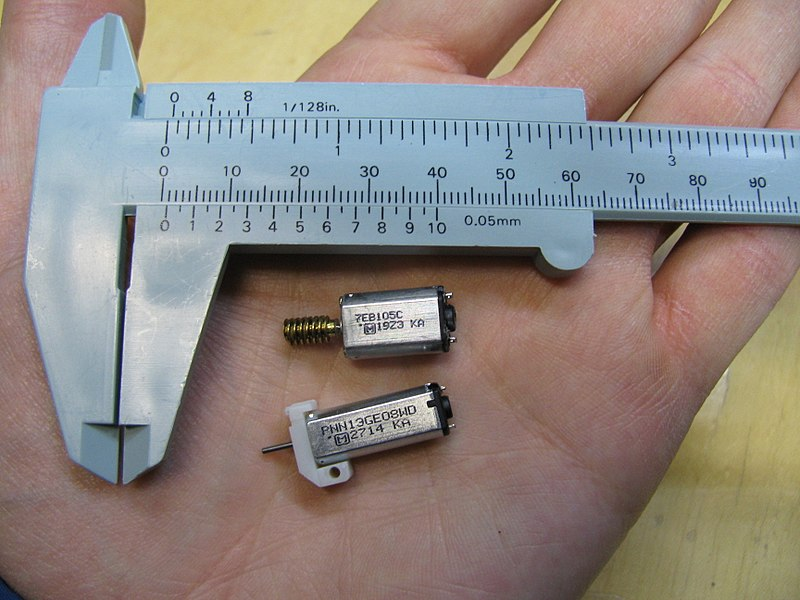
\includegraphics[height=0.6\textheight]{../../figures/wiki-small-dc-motor.jpg}
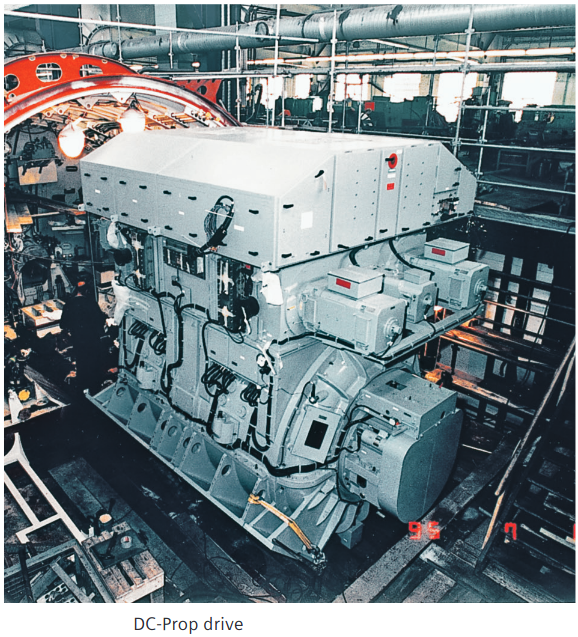
\includegraphics[width=0.6\textheight]{../../figures/Siemens-DC-prop.png}\\
{\footnotesize Fuente: Wikipedia \hspace*{3cm} Fuente: Siemens AG}
\end{center}
\end{frame}


\begin{frame}[label={sec:org7c40f0d}]{Fuerza en un conductor eléctrico en un campo magnético}
\begin{center}
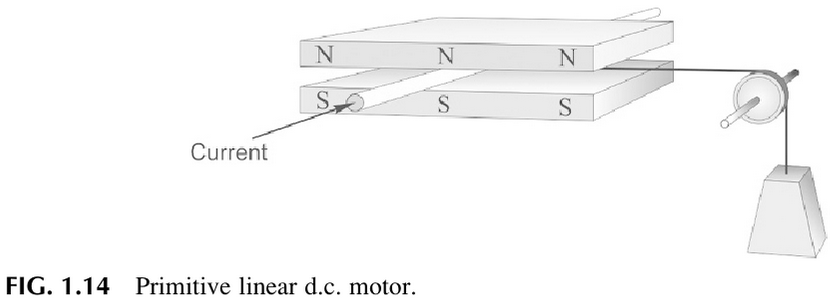
\includegraphics[width=0.4\linewidth]{../../figures/HD-fig1_14.png}
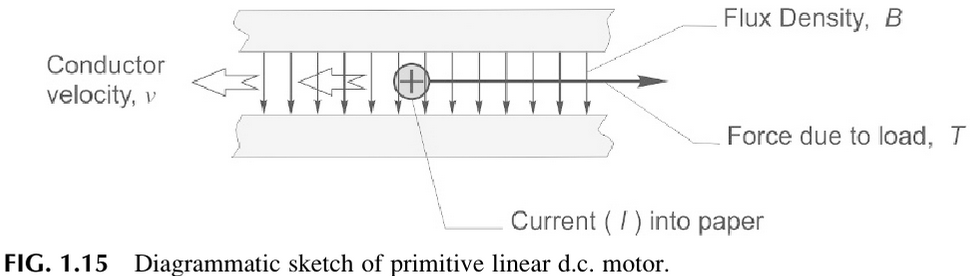
\includegraphics[width=0.53\linewidth]{../../figures/HD-fig1_15.png}
\end{center}


\begin{block}{Fuente}
\begin{center}
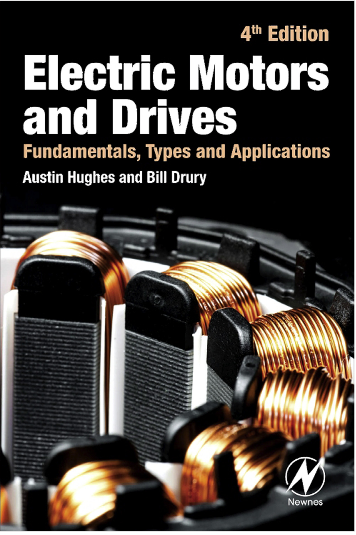
\includegraphics[width=0.2\linewidth]{../../figures/textbook.png}
\end{center}
\end{block}
\end{frame}


\begin{frame}[label={sec:orgce9e7b6}]{Fuerza en un conductor eléctrico en un campo magnético}
\begin{center}
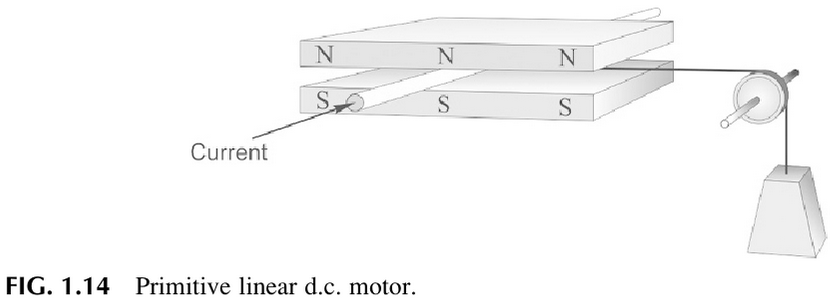
\includegraphics[width=0.4\linewidth]{../../figures/HD-fig1_14.png}
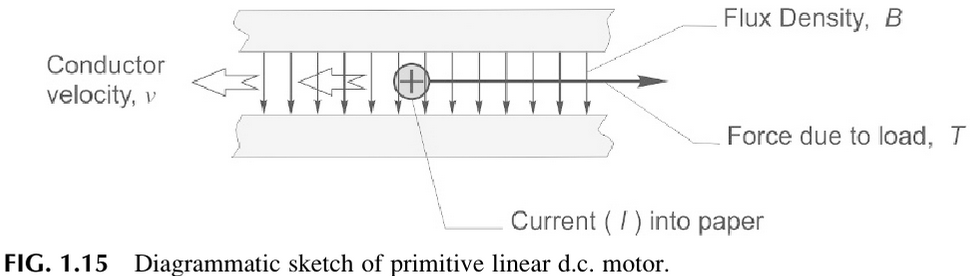
\includegraphics[width=0.53\linewidth]{../../figures/HD-fig1_15.png}
\end{center}

La fuerza electromagnética en el conductor es \alert{proporcional a la corriente}:
\[F=k_mI=(Bl_m)I,\] donde \(B\) es la densidad del flujo magnético en el entrehierro, \(I\) es la corriente, y \(l_m\) es la longitud del cable. En vez de construir un motor muy larga, se agreaga varias cables juntos para aumentar la fuerza.

\alert{Actividad individual 4} En un motor grande de \unit{4}{\mega\watt} con longitud axial de \(l_m=\unit{2}{\meter}\), la densidad del flujo es \(B=\unit{0.8}{\tesla}\) y la corriente es \(I=\unit{3}{\kilo\ampere}\). ¿Cuantas cables en paralelo se necesita para alcanzar una fuerza de \(F=\unit{259.2}{\kilo\newton}\)?
\end{frame}

\begin{frame}[label={sec:org2f27d94}]{Las dos ecuaciónes del motor eléctrica CC}
\begin{block}{Fuerza generado en el conductor por la corriente en el campo magnético}
\[ F(t) = k_m i(t) \quad\Leftrightarrow\quad T(t) = k_m r i(t),\]
dónde \(r\) es el radie del motor.
\end{block}

\begin{block}{Voltaje generado por el movimiento del conductor en el campo magnético}
\[ e(t) = k_v v(t) \quad\Leftrightarrow\quad e(t) = k_v r \omega(t)\]
\(e(t)\) se llama \emph{Fuerza contraelectromotriz} o \emph{Back electro-motive force (Back e.m.f.)} en inglés.
\end{block}
\end{frame}
\begin{frame}[label={sec:org9a1ab45}]{Potencia eléctrica y mecánica}
\begin{center}
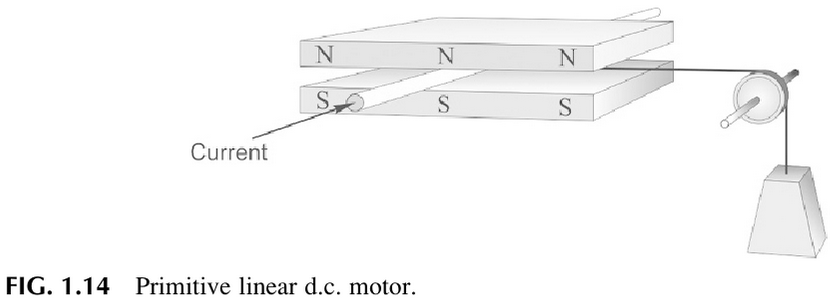
\includegraphics[width=0.4\linewidth]{../../figures/HD-fig1_14.png}
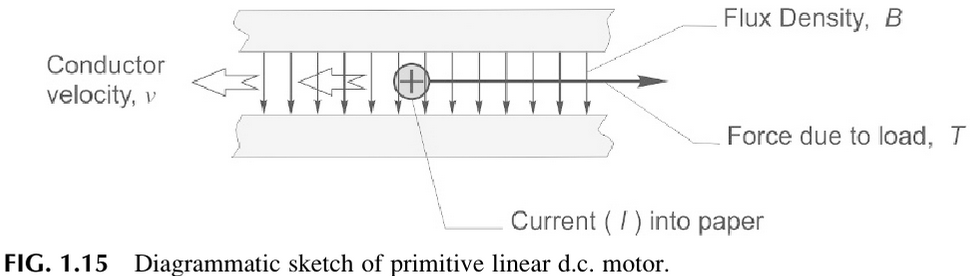
\includegraphics[width=0.53\linewidth]{../../figures/HD-fig1_15.png}
\end{center}

Con velocidad \(v\) constante y ignorando fricción y resistencia eléctrica: 

\[ \text{Fuerza electromagnética} = \text{Fuerza mecánica} \quad\Leftrightarrow\quad F=k_mI =Bl_mI = mg\]
\[ \text{Potencia eléctrica} = \text{Potencia mecánica} \quad \Leftrightarrow\quad \underbrace{V_1I}_{P_e} = \underbrace{Fv = Bl_mI v}_{P_m} \] 
Se necesita aplicar un voltaje \(V_1\) sobre el cable para mantener la corriente \(I\). \alert{Ese voltaje es igual al back e.m.f.} 
\[ V_1I = Bl_mIv \quad \Rightarrow \quad V_1 = (Bl_m)v = k_v v = \tikz[baseline = 0.1ex]{\node[red, circle, draw, inner sep=3pt, pin={[red]0:{Back e.m.f.}}] at (0, 0.1 cm) {\textcolor{black}{E}}}\]

\alert{Actividad individual 5} ¿Cuál es la relación entre los dos constantes, \(k_m\) y \(k_v\)?
\end{frame}

\begin{frame}[label={sec:org720bb2a}]{Potencia eléctrica y mecánica}
En realidad se pierde parte de la energía por la resistencia en el circuito eléctrico.
\begin{align*}
\text{Potencia eléctrica aplicada} &= \text{Producción de calor} + \text{Potencia mecánica}\\
V_2 I &= RI^2 + EI
\end{align*}
Dónde \(V_2 > V_1 = (Bl_m)v = E\).

La eficiencia del motor

\[ \text{eficiencia} = \frac{\text{Potencia mecánica}}{\text{Potencia eléctrica aplicada}} = \frac{EI}{V_2I} = \frac{E}{RI + E}\]

\alert{Ejercicio} Un motor eléctrico tiene el constante \(k=\unit{0.05}{\kilo\newton\per\ampere}\) y una resistencia de \(R=\SI{2}{\milli\ohm}\). Está produciendo una potencia mecánica de \unit{4}{\mega\watt} a una velocidad de \(v=\unit{10}{\meter\per\second}\) Calcula el 'back e.m.f' \(E\), la corriente \(I\), el voltaje \(V_2\) y la eficiencia.
\end{frame}

\begin{frame}[label={sec:org43f9ec3}]{Potencia eléctrica y mecánica}
\begin{block}{Equilibrio de energía}
\begin{align*}
\text{Potencia eléctrica aplicada} &= \text{Producción de calor} + \text{Potencia mecánica}\\
V_2 I &= RI^2 + EI
\end{align*}
\end{block}
\begin{block}{Eficiencia}
\[ \text{eficiencia} = \frac{\text{Potencia mecánica}}{\text{Potencia eléctrica aplicada}} = \frac{V_2}{RI + E}\]

\alert{Actividad en pares} En el ejemplo anterior el motor tenía un constante de \(k=\unit{0.05}{\kilo\newton\per\ampere}\). Supone que otro motor con la misma resistancia \(R=\SI{2}{\milli\ohm}\) está haciendo el mismo trabajo (\unit{4}{\mega\watt} a \unit{10}{\meter\per\second}), pero tiene el konstante \(k=\unit{0.1}{\kilo\newton\per\ampere}\). ¿Cuál es su eficiencia?
\end{block}
\end{frame}


\begin{frame}[label={sec:orgc4cb3eb}]{Rotación}
\begin{center}
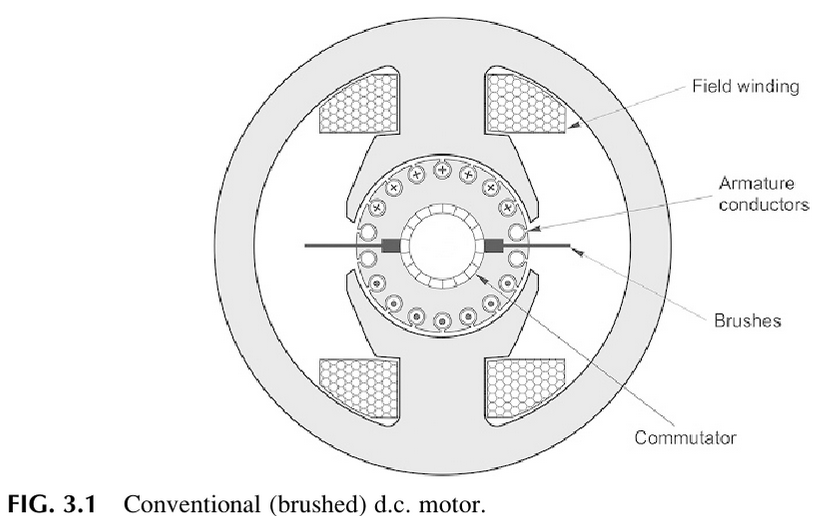
\includegraphics[width=0.4\linewidth]{../../figures/HD-fig3_1.png}
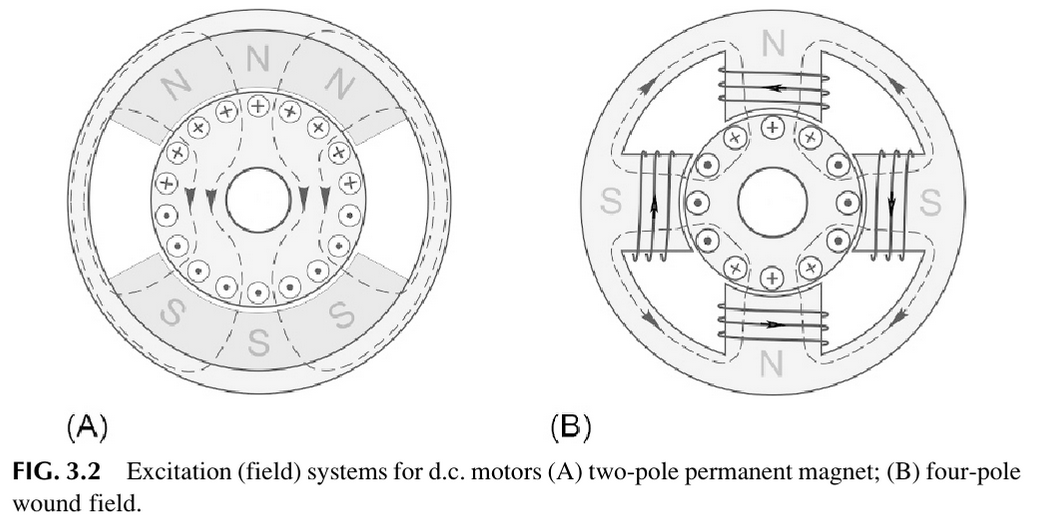
\includegraphics[width=0.53\linewidth]{../../figures/HD-fig3_2.png}
{\footnotesize Funte: Hughes and Drury}
\end{center}
\end{frame}

\begin{frame}[label={sec:orge92d287}]{Circuito equivalente}
\begin{center}
  \begin{circuitikz}
    \draw (4,1) node[elmech](motor){M};
    \draw (motor.north) to[R=$R$] (4,4) to[L=$L$] (0,4)
    to[american voltage source, label=$V$] (0,0) -| (motor.south);
    \draw[thick,->>](motor.right)--++(1,0)node[midway,above]{$\omega$};

    \node[] at (2, -0.8 cm) {\(L \frac{d}{dt}i(t) +  Ri(t) + k\omega(t) = V\)};

    \begin{scope}[xshift=8cm]
    \draw (4,1) node[elmech](motor){M};
    \draw (motor.north) to[R=$R$] (4,4) to[short] (0,4)
    to[american voltage source, label=$V$] (0,0) -| (motor.south);
    \draw[thick,->>](motor.right)--++(1,0)node[midway,above]{$\omega$};
    \node[] at (2, -0.8 cm) {\(Ri(t) + k\omega(t) = V\)};
    \end{scope}
  \end{circuitikz}
\end{center}

\begin{center}
Newton: \(J\frac{d}{dt}\omega(t) = ki(t) - T_l(t)\)
\end{center}
\end{frame}


\begin{frame}[label={sec:orgd4ed1dc}]{Velocidad con carga constante}
\begin{align}
L\frac{d}{dt}i(t) + Ri(t) + k\omega(t) &= V(t)\\
J\frac{d}{dt}\omega(t) &= ki(t) - T_l(t)
\end{align}

En estado estable: \(i(t) = I\), \(\omega(t) = \omega\).

\begin{align}
RI + k\omega &= V\\
0 &= kI - T_l
\end{align}

\alert{Actividad individual 6} Escribe la velocidad angular como función de la carga \(T_l\) y el voltaje \(V\)
\[\omega = f(V, T_l) = \frac{V}{k} - \frac{RT_l}{k^2}\]
\end{frame}

\begin{frame}[label={sec:org03e5f51}]{Velocidad con carga constante}
\[\omega = f(V, T_l) = \frac{V}{k} - \frac{RT_l}{k^2}\]
Un motor especifico tiene el constante \(k=\unit{4}{\newton\meter\per\ampere}\) y resistencia \(R=\SI{1}{\ohm}\). Se aplica un voltaje de \(V=\unit{100}{\volt}\) sobre su armadura.


\alert{Actividad en pares} Dibuje como la velocidad en estado estable depende de la carga \(T_l\). ¿Cuál es el par de parada?

\begin{center}
  \begin{tikzpicture}[xscale=0.8]
    \draw[->] (0, 0) -- (9, 0) node[right] {$T_l$ [\unit{}{\newton\meter}]};
    \draw[->] (0, 0) -- (0, 3) node[left] {$\omega$};
    \foreach \t in { 1, 2, ..., 8} {
    \draw (\t, 0) -- (\t, -0.1) node[below] {\t{}00};
    }
    \end{tikzpicture}

\end{center}
\end{frame}

\begin{frame}[label={sec:org8fee989}]{Arranque}
Para un motor parada, la fuerza contraelectromotriz es cero, y solo la resistencia y la inductancia de la armadura limiten la corriente.

\begin{center}
  \begin{circuitikz}
    \draw (4,1) node[elmech](motor){M};
    \draw (motor.north) to[R=$R$] (4,4) to[L=$L$] (0,4)
    to[american voltage source, label=$V$] (0,0) -| (motor.south);
    \draw[thick,->>](motor.right)--++(1,0)node[midway,above]{$\omega$};

    \node[] at (2, -0.8 cm) {\(L \frac{d}{dt}i(t) +  Ri(t) + k\omega(t) = V\)};
  \end{circuitikz}
\end{center}


Hay que tener cuidado en el arranque para que la corriente no sube a niveles excedentes.
\end{frame}

\section{Modeling}
\label{sec:orgb895451}
\begin{frame}[label={sec:org5be9ad8}]{Modelo de bloques del circuito equivalente}
\begin{center}
  \begin{circuitikz}
    \draw (4,1) node[elmech](motor){M};
    \draw (motor.north) to[R=$R$] (4,4) to[L=$L$] (0,4)
    to[american voltage source, label=$V$] (0,0) -| (motor.south);
    \draw[thick,->>](motor.right)--++(1,0)node[midway,above]{$\omega$};

    \node[] at (9, 2 cm) {\(L \frac{d}{dt}i(t) +  Ri(t) + k\omega(t) = V\)};
    \node[] at (9, 1 cm) {\(\frac{d}{dt}i(t) = \frac{1}{L} \Big(-Ri(t) - k\omega(t) + V\Big)\)};
  \begin{scope}[yshift=-15mm, xshift=6cm,
  block/.style={rectangle, draw, minimum width=12mm, minimum height=10mm},
  amp/.style = {regular polygon, regular polygon sides=3,
        draw, fill=white, text width=1em,
        inner sep=1pt, outer sep=0mm,
        shape border rotate=-90},
	summ/.style = {circle, draw, inner sep = 1pt},]
   \node[block,] (int) at (0,0) {$\int$};
   \node[amp, left of=int, node distance=40mm] (oneoverL) {$\frac{1}{L}$}; 
   \draw[->] (oneoverL) -- node[above] {$\frac{d}{dt}i(t)$} (int);
   \node[summ, left of=oneoverL] (sum) {\small $\Sigma$};
   \end{scope}
  \end{circuitikz}
  \end{center}
\end{frame}
\end{document}